\documentclass[11pt]{article}
\usepackage[margin=1in]{geometry}
\usepackage{amsmath,amssymb,amsthm,mathtools}
\usepackage{booktabs,tabularx,enumitem,microtype,xcolor}
\usepackage{tikz}
\usetikzlibrary{arrows.meta,positioning}
\usepackage[colorlinks=true,linkcolor=blue!45!black,citecolor=blue!45!black,urlcolor=blue!45!black]{hyperref}
\hypersetup{pdftitle={No binary [[16,5,5]] stabilizer code exists},pdfauthor={Brandon Li}}
\setlength{\parindent}{0pt}
\setlength{\parskip}{5pt plus 1pt minus 1pt}
\setlength{\emergencystretch}{2em}
\setlength{\belowcaptionskip}{6pt}
\setlist{nosep,leftmargin=*}

\newtheorem{theorem}{Theorem}[section]
\newtheorem{proposition}[theorem]{Proposition}
\newtheorem{lemma}[theorem]{Lemma}
\newtheorem{corollary}[theorem]{Corollary}
\theoremstyle{definition}
\newtheorem{definition}[theorem]{Definition}
\theoremstyle{remark}
\newtheorem{remark}[theorem]{Remark}

\newcommand{\F}{\mathbb F_2}
\newcommand{\qc}[1]{[\![#1]\!]}
\newcommand{\wt}{\operatorname{wt}}
\newcommand{\cost}{c}
\newcommand{\Sh}{\mathrm{Sh}}
\newcommand{\tr}{\mathsf T}
\newcommand{\Aut}{\operatorname{Aut}}
\newcommand{\pathcode}[1]{{\small\nolinkurl{#1}}}

\title{No binary \(\qc{16,5,5}\) stabilizer code exists}
\author{Brandon Li\\[0.2em]
\normalsize John L. Miller Great Neck North High School, Great Neck, New York\\
\normalsize\href{mailto:brandon.li.gn@gmail.com}{brandon.li.gn@gmail.com}}
\date{November 2026}

\begin{document}
\maketitle

\begin{abstract}
We prove that no binary stabilizer code with parameters \(\qc{16,5,5}\)
exists, pure or degenerate. Since a \(\qc{16,5,4}\) code is known, the
largest distance of a binary \(\qc{16,5}\) stabilizer code is \(4\),
which settles an open entry in Grassl's tables. Integer certificates for
refined weight enumerators show first that such a code would be pure
and that its lightest nonzero stabilizer would have weight between \(6\)
and \(9\). Shortening the code on the support of a lightest stabilizer
leaves a small additive code, which must lie in one of \(3{,}957\)
equivalence classes, and ties the rest of the code to a linear map that
has to satisfy a simple weight condition. A complete computer search,
carried out by two separately written methods for every class, shows
that no such map exists.
\end{abstract}

\textbf{Keywords:} quantum error correction; stabilizer codes; additive
codes; nonexistence; shortening; computer-assisted proof.

%=====================================================================
\section{Introduction}\label{sec:intro}

An \(\qc{n,k,d}\) quantum code uses \(n\) physical qubits to store \(k\)
logical qubits. Its minimum distance \(d\) is the smallest number of
qubits on which a Pauli operator can act nontrivially on the encoded
information while commuting with every stabilizer, and a code of
distance \(d\) corrects arbitrary errors on up to \(\lfloor
(d-1)/2\rfloor\) qubits. Let \(d_{\max}(n,k)\) be the largest minimum
distance of a binary stabilizer code with \(n\) physical and \(k\)
logical qubits. For small \(n\) and \(k\), Grassl's tables
\cite{grassl} record the best distance known to be achievable and the
best upper bound known. Where the two numbers differ the question is
open: either a better code exists and has not yet been found, or one
has to prove that it cannot exist.

This paper settles the case \((n,k)=(16,5)\). The table lists a
\(\qc{16,5,4}\) code, obtained by extending a \(\qc{14,5,4}\) code by two
coordinates, while the linear programming bound still allows distance
five. So before this work \(4\leq d_{\max}(16,5)\leq5\). We show that
distance five is impossible.

\begin{theorem}\label{thm:main}
There is no binary stabilizer code with parameters \(\qc{16,5,d}\) for
any \(d\geq5\). Hence \(d_{\max}(16,5)=4\).
\end{theorem}

The theorem covers degenerate codes as well as pure ones: we prove that
such a code would have to be pure, rather than assuming it. It is a
statement about stabilizer (additive) codes; nonadditive codes are not
considered.

Several recent methods bear on this case without deciding it. The
semidefinite programming bounds of Angl\`es Munn\'e and Huber \cite{sdp}
apply to all codes; their Table~1 gives \(32\leq K\leq 42\) for the
code-space dimension at \((n,d)=(16,5)\), so \(K=2^5=32\) is not
excluded. Lai \cite{lai} develops refined weight-enumerator tests, and
his Section~VII-D still leaves 27 candidate weight distributions for a
\(\qc{16,5,5}\) code. Our argument instead combines weight-enumerator
certificates with a structural reduction and a finite search, in the
spirit of the proof by Bierbrauer et al.\ \cite{bierbrauer} that no
\(\qc{13,5,4}\) code exists. It relies on the classification of small
additive codes of distance five by Grassl, Krotov, Sok and Sol\'e
\cite{dodeca}, and on the standard symplectic description of stabilizer
codes together with the MacWilliams and shadow identities
\cite{crss,rains}. The same method also shows that no \(\qc{17,3,6}\)
code exists; that proof is given separately.

\subsection*{The idea of the proof}

The proof is by contradiction. Suppose \(S\) is a \(\qc{16,5,5}\) code.
The argument has three steps, shown in Figure~\ref{fig:flow}.

\emph{Step 1: no light stabilizers.} A code of distance five may still
contain stabilizers of weight less than five, so we first rule these
out. We refine the weight enumerator of \(S\) by fixing a light
stabilizer and recording, for every word, its weight on the support of
that stabilizer and its weight elsewhere. The MacWilliams and shadow
identities then give linear systems with no nonnegative solution. Each
infeasibility comes with integer multipliers that combine the
constraints into an impossible inequality, and these can be checked
with exact arithmetic. Together with one congruence modulo \(4096\),
they show that \(S\) is pure and that its lightest nonzero stabilizer
has some weight \(m\) between \(6\) and \(9\).

\emph{Step 2: cut the code in two.} Fix a stabilizer \(p\) of weight
\(m\), and let \(T\) be the set of qubits where it acts. The centralizer
words that act only outside \(T\) form an additive code \(C\) of length
\(16-m\), and its parameters are forced. Codes this small have been
classified: up to equivalence there are \(3{,}957\) of them, and we
rebuild the list ourselves and check that it is complete. The remaining
centralizer words are described by a linear map \(M\) from a
\((2m-2)\)-dimensional space of operators on \(T\) to the \(1024\)
cosets of \(C\). The distance of \(S\) becomes a condition on \(M\): an
operator on \(T\) of weight \(c\) must be sent to a coset whose lightest
word has weight at least \(5-c\).

\emph{Step 3: search every class.} For each of the \(3{,}957\) codes
\(C\), a computer searches for a linear map \(M\) that meets the
condition, and finds none. Every class is searched twice, by two
separately written methods, and each program does find the map that
comes from a known \(\qc{16,4,5}\) code when it is given that code.

Section~\ref{sec:prelim} fixes notation. Steps 1, 2 and 3 are carried
out in Sections~\ref{sec:purity}, \ref{sec:shorten}--\ref{sec:map} and
\ref{sec:search}. Section~\ref{sec:proof} puts the pieces together and
describes how to rerun every computation.

\begin{figure}[htbp]
\centering
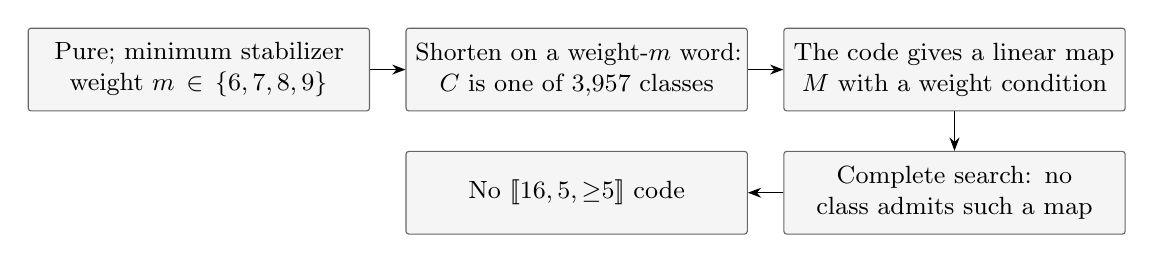
\begin{tikzpicture}[>=Stealth,
 box/.style={draw=black!60,fill=black!4,rounded corners=1pt,
 text width=4.1cm,minimum height=1.05cm,align=center,font=\small},
 node distance=0.5cm and 0.45cm]
\node[box] (a) {Pure; minimum stabilizer weight \(m\in\{6,7,8,9\}\)};
\node[box,right=of a] (b) {Shorten on a weight-\(m\) word:\\ \(C\) is one of \(3{,}957\) classes};
\node[box,right=of b] (c) {The code gives a linear map \(M\) with a weight condition};
\node[box,below=of c] (d) {Complete search: no class admits such a map};
\node[box,left=of d] (e) {No \(\qc{16,5,{\geq}5}\) code};
\draw[->] (a)--(b); \draw[->] (b)--(c); \draw[->] (c)--(d); \draw[->] (d)--(e);
\end{tikzpicture}
\caption{Structure of the proof.}
\label{fig:flow}
\end{figure}

%=====================================================================
\section{Preliminaries}\label{sec:prelim}

We use the binary symplectic description of Pauli operators
\cite{crss}. All vector spaces are over \(\F\), and
\[
 V_n=\F^{2n}=\{(x\mid z):x,z\in\F^n\},\qquad
 \langle (x\mid z),(x'\mid z')\rangle=x\cdot z'+z\cdot x'.
\]
At each coordinate the pairs \((0,0),(1,0),(0,1),(1,1)\) stand for the
Pauli letters \(I,X,Z,Y\). Adding vectors corresponds to multiplying
Pauli operators up to phase, and the symplectic product is \(0\) when
two operators commute and \(1\) when they anticommute. The weight
\(\wt(x\mid z)\) is the number of coordinates whose letter is not \(I\),
and we write \(\varepsilon(v)=\wt(v)\bmod 2\).

A subspace is isotropic if all its symplectic products vanish. A binary
\(\qc{n,k}\) stabilizer code is an isotropic subspace \(S\leq V_n\) of
dimension \(n-k\). Its centralizer \(S^\perp\) has dimension \(n+k\) and
contains \(S\). For \(k>0\) the minimum distance is
\(d=\min\{\wt(v):v\in S^\perp\setminus S\}\). The code is \emph{pure to
distance \(\delta\)} if every nonzero word of \(S^\perp\) has weight at
least \(\delta\); for a code of distance at least \(\delta\) this means
that no nonzero stabilizer word has weight below \(\delta\). We call the
elements of \(S\) stabilizer words and write \(A_w\) for the number of
them of weight \(w\).

We also need codes that are not isotropic. An additive code of length
\(\ell\) is any subspace \(C\leq V_\ell\). It is an
\((\ell,2^c,{\geq}\delta)_4\) code if \(\dim C=c\), so that \(C\) has
\(2^c\) words over the four-letter Pauli alphabet, and every nonzero
word has weight at least \(\delta\). Two additive codes are
\emph{equivalent} if a permutation of coordinates followed by an
invertible \(\F\)-linear map of \(\F^2\) at each coordinate carries one
to the other. Since \(\mathrm{GL}(2,2)\) permutes the three nonzero
letters and equals \(\mathrm{Sp}(2,2)\), these maps preserve both weight
and the symplectic form. On stabilizer codes they are the local Clifford
operations combined with qubit permutations, and they send an
\(\qc{n,k,d}\) code to an \(\qc{n,k,d}\) code with the same weight
enumerator. In particular, any stabilizer word of weight \(w\) can be
moved to \(Z^w=Z\otimes\cdots\otimes Z\) on the first \(w\) qubits.

For a set \(T\) of coordinates, \(V_T\leq V_n\) denotes the words that
are \(I\) outside \(T\), and \(W=V_{T^c}\) the words that are \(I\) on
\(T\), so that \(V_n=V_T\oplus W\). We write \(\pi_T\) for restriction
to \(T\) and identify \(W\) with \(V_{n-|T|}\) when convenient. Two
facts are used repeatedly.

\begin{lemma}[Weight parity]\label{lem:parity-linear}
For all \(u,v\in V_n\),
\(\varepsilon(u+v)=\varepsilon(u)+\varepsilon(v)+\langle u,v\rangle\).
In particular \(\varepsilon\) is linear on every isotropic subspace.
\end{lemma}
\begin{proof}
It suffices to check one coordinate, with letters \(\alpha,\beta\in\F^2\).
If \(\alpha=0\) or \(\beta=0\), then \(\langle\alpha,\beta\rangle=0\)
and \(\wt(\alpha+\beta)=\wt(\alpha)+\wt(\beta)\), so both sides agree.
If \(\alpha=\beta\ne0\), the left side is \(\varepsilon(0)=0\) and the
right side is \(1+1+0\equiv0\). If \(\alpha\ne\beta\) are both nonzero,
then \(\alpha+\beta\) is the third nonzero letter, so the left side is
\(1\); two distinct nonidentity Pauli letters anticommute, so the right
side is \(1+1+1\equiv1\).
\end{proof}

\begin{lemma}[Shortening]\label{lem:shorten}
Let \(S\) be an \(\qc{n,k}\) code that is pure to distance \(\delta\).
Let \(T\) be a set of \(m\) coordinates, \(R=S\cap V_T\) and
\(r=\dim R\). Then \(\pi_T(S^\perp)=R^\perp\cap V_T\), and
\(C=S^\perp\cap W\) is an additive \((n-m,2^{n+k-2m+r},{\geq}\delta)_4\)
code.
\end{lemma}
\begin{proof}
A word \(u\in V_T\) is orthogonal to \(\pi_T(S^\perp)\) if and only if it
is orthogonal to \(S^\perp\), that is, \(u\in S\cap V_T=R\). Hence the
annihilator of \(\pi_T(S^\perp)\) inside \(V_T\) is \(R\), so
\(\pi_T(S^\perp)=R^\perp\cap V_T\), of dimension \(2m-r\). The kernel of
\(\pi_T\) on \(S^\perp\) is \(C\), so \(\dim C=(n+k)-(2m-r)\). Nonzero
words of \(C\) are nonzero words of \(S^\perp\), so they have weight at
least \(\delta\).
\end{proof}

%=====================================================================
\section{Purity and the minimum stabilizer weight}\label{sec:purity}

From now on \(S\) is a hypothetical \(\qc{16,5,{\geq}5}\) code, so
\(|S|=2^{11}=2048\). Distance five forbids light logical operators, but
not light stabilizers: a degenerate code could contain stabilizer words
of weight below five. This section shows that it does not, and that the
lightest nonzero stabilizer word has weight between \(6\) and \(9\).
The tool is linear programming on a refined weight enumerator, made
rigorous by integer certificates.

\subsection{Split weight enumerators}

Suppose \(S\) contains a word of weight \(w\in\{1,\ldots,5\}\). After a
local Clifford operation it is \(r=Z^w\) on the block \(B\) of the first
\(w\) qubits. Put \(f=16-w\) and \(R=\langle r\rangle\leq S\). We sort
the words of \(S\) by their weight on \(B\) and their weight on the
other \(f\) qubits, and do so through the cosets of \(R\). Each coset
\(s+R\subseteq S\) has a fixed restriction to the other \(f\) qubits, of
some weight \(b\), and its restriction to \(B\) is a coset of \(R\)
inside \(R^\perp\cap V_B\). The \emph{pattern} of that local coset is
\(P=(P_0,\ldots,P_w)\), where \(P_a\) counts its two elements of weight
\(a\). Let \(\mathcal P_w\) be the set of distinct patterns of the
\(2^{2w-2}\) cosets of \(R\) in \(R^\perp\cap V_B\); Table~\ref{tab:patterns}
lists them. For example, for \(w=2\) the words commuting with \(ZZ\) are
those whose two letters both lie in \(\{I,Z\}\) or both lie in
\(\{X,Y\}\), and the four cosets of \(R\) are \(\{II,ZZ\}\),
\(\{ZI,IZ\}\), \(\{XX,YY\}\) and \(\{XY,YX\}\), with patterns
\((1,0,1)\), \((0,2,0)\), \((0,0,2)\) and \((0,0,2)\).

\begin{table}[h!]
\centering\small
\caption{The coset patterns \(\mathcal P_w\). Each entry is a pattern
\((P_0,\ldots,P_w)\), followed by the number of cosets of \(R\) in
\(R^\perp\cap V_B\) that have it.}\label{tab:patterns}
\begin{tabular}{@{}cl@{}}\toprule
\(w\)&Patterns\\\midrule
1&\((1,1)\times1\)\\
2&\((1,0,1)\times1,\ (0,2,0)\times1,\ (0,0,2)\times2\)\\
3&\((1,0,0,1)\times1,\ (0,1,1,0)\times3,\ (0,0,1,1)\times12\)\\
4&\((1,0,0,0,1)\times1,\ (0,1,0,1,0)\times4,\ (0,0,2,0,0)\times3,\)\\
 &\((0,0,1,0,1)\times24,\ (0,0,0,2,0)\times24,\ (0,0,0,0,2)\times8\)\\
5&\((1,0,0,0,0,1)\times1,\ (0,1,0,0,1,0)\times5,\ (0,0,1,1,0,0)\times10,\)\\
 &\((0,0,1,0,0,1)\times40,\ (0,0,0,1,1,0)\times120,\ (0,0,0,0,1,1)\times80\)\\\bottomrule
\end{tabular}
\end{table}

The unknowns are the numbers \(x_{P,b}\geq0\), one for each
\(P\in\mathcal P_w\) and \(b\in\{0,\ldots,f\}\), counting the cosets of
\(R\) in \(S\) with pattern \(P\) and outside weight \(b\). The split
enumerator
\[
 H_{a,b}=\sum_{P}P_a\,x_{P,b}
\]
then counts the words of \(S\) with weight \(a\) on \(B\) and \(b\)
outside. In the last case below there is no block: \(w=0\), \(f=16\),
and the unknowns are simply \(x_b=A_b\).

The split enumerator of \(S\) determines those of the centralizer and
of the shadow. With the quaternary Krawtchouk polynomials
\(K^\ell_a(i)=[u^a]\,(1+3u)^{\ell-i}(1-u)^i\), put
\[
 T_{a,b}=\sum_{a',b'}K^w_a(a')K^f_b(b')H_{a',b'},\qquad
 \Sigma_{a,b}=\sum_{a',b'}(-1)^{a'+b'}K^w_a(a')K^f_b(b')H_{a',b'}.
\]
Summing the character identity \(\mathbf 1[v\in S^\perp]=2^{-11}
\sum_{s\in S}(-1)^{\langle v,s\rangle}\) over all \(v\) of split weight
\((a,b)\) shows that \(T_{a,b}/2^{11}\) is the number of centralizer
words of split weight \((a,b)\); this is the split MacWilliams identity.
By Lemma~\ref{lem:parity-linear}, \(\varepsilon\) is a linear functional
on \(S\), so the \emph{shadow}
\(\{v:\langle v,s\rangle=\varepsilon(s)\text{ for all }s\in S\}\) is a
coset of \(S^\perp\). The same computation with
\((-1)^{\langle v,s\rangle+\varepsilon(s)}\) shows that
\(\Sigma_{a,b}/2^{11}\) counts the shadow words of split weight
\((a,b)\) \cite{rains}, so it cannot be negative.

\subsection{The linear systems and their certificates}

Every \(\qc{16,5,{\geq}5}\) code containing \(r\) satisfies the
following constraints. We give each a name, which the certificate list
below refers to.
\begin{enumerate}[label=(\roman*)]
\item \(U\): \(H_{0,0}=1\), and \(N\): \(\sum_{a,b}H_{a,b}=2^{11}\);
\item \(L_{a,b}\): \(T_{a,b}-2^{11}H_{a,b}=0\) for \(1\leq a+b\leq4\),
 because every centralizer word of weight at most four is a stabilizer
 word;
\item \(\Sigma_{a,b}\): \(-\Sigma_{a,b}\leq0\) for all \(a,b\);
\item the hypotheses of the case being treated: \(A_j\):
 \(\sum_{a+b=j}H_{a,b}=0\), or \(A_4^{\geq2}\):
 \(-\sum_{a+b=4}H_{a,b}\leq-2\).
\end{enumerate}
In case (d) there is no block, \(H_b=A_b\), and the rows are named
\(L_b\), \(A_j\) in the same way. None of these constraints assumes
purity. The constraint \(H_{0,0}=1\) also records that \(r\in S\): the
only coset of \(R\) in \(R^\perp\cap V_B\) that contains a weight-zero
word is \(R=\{I^w,Z^w\}\) itself, so its pattern is the only one with
\(P_0>0\), and \(H_{0,0}=1\) forces exactly one coset of \(S\) with that
pattern and outside weight \(0\), namely \(R\).

Write the system as \(Ex=e\), \(Gx\leq g\), \(x\geq0\). To show it has
no solution we exhibit an \emph{infeasibility certificate}: integer
multiplier vectors \(\nu\) (of any sign) and \(\lambda\geq0\) such that
the combined row \(c=\nu E+\lambda G\) has every coefficient
\(c\geq0\) while \(\nu e+\lambda g<0\). A feasible \(x\) would give
\(0\leq cx\leq \nu e+\lambda g<0\), which is impossible. Checking a
certificate needs only exact integer arithmetic, however the
multipliers were found.

\begin{proposition}\label{prop:certs}
Each of the following cases has an infeasibility certificate, so none
of them occurs for a \(\qc{16,5,{\geq}5}\) code:
\begin{enumerate}[label=(\alph*)]
\item \(S\) contains a word of weight \(1\), \(2\) or \(3\);
\item \(S\) contains a word of weight \(4\) and \(A_4\geq2\);
\item \(A_1=\cdots=A_4=0\) and \(S\) contains a word of weight \(5\);
\item \(A_1=\cdots=A_9=0\).
\end{enumerate}
\end{proposition}

There are six certificates, summarized in Table~\ref{tab:certs} and
listed in full below. Our checker rebuilds every row from its name,
recomputes the patterns \(\mathcal P_w\) by enumerating
\(R^\perp\cap V_B\), and verifies both sign conditions in exact integer
arithmetic.

\begin{table}[h!]
\centering\small
\caption{The six infeasibility certificates. ``Columns'' is the number
of variables, ``rows'' the number of rows with a nonzero multiplier, and
the last column is \(\nu e+\lambda g\). In case (d) there is no block,
and the 17 variables are \(A_0,\ldots,A_{16}\).}\label{tab:certs}
\begin{tabular}{@{}llrrr@{}}\toprule
Case&Assumption&Columns&Rows&Right-hand side\\\midrule
(a)&\(S\ni Z\)&16&6&\(-11{,}520\)\\
(a)&\(S\ni ZZ\)&45&14&\(-374{,}784\)\\
(a)&\(S\ni Z^3\)&42&15&\(-5{,}662{,}720\)\\
(b)&\(S\ni Z^4\), \(A_4\geq2\)&78&26&\(-7{,}294{,}976\)\\
(c)&\(S\ni Z^5\), \(A_1=\cdots=A_4=0\)&72&24&\(-8{,}192\)\\
(d)&\(A_1=\cdots=A_9=0\)&17&15&\(-61{,}440\)\\\bottomrule
\end{tabular}
\end{table}

In the list, each entry is the multiplier of one named row; rows without
an entry have multiplier zero, and the multipliers \(\lambda\) of
inequality rows are positive. With Table~\ref{tab:patterns} the rows can
be rebuilt from their names, so the reader can check both sign
conditions with any computer algebra system.
{\small\raggedright
\begin{description}[leftmargin=1.5em,style=nextline]
\item[(a), \(S\ni Z\)] \mbox{\(\nu(U)=-349{,}440\)}, \mbox{\(\nu(N)=165\)}, \mbox{\(\nu(L_{0,4})=1\)}, \mbox{\(\nu(L_{1,1})=36\)}, \mbox{\(\nu(L_{1,2})=14\)}, \mbox{\(\nu(L_{1,3})=4\)}.
\item[(a), \(S\ni ZZ\)] \mbox{\(\nu(U)=-3{,}741{,}696\)}, \mbox{\(\nu(N)=1{,}644\)}, \mbox{\(\nu(L_{0,1})=221\)}, \mbox{\(\nu(L_{0,2})=193\)}, \mbox{\(\nu(L_{0,3})=33\)}, \mbox{\(\nu(L_{0,4})=15\)}, \mbox{\(\nu(L_{1,0})=-57\)}, \mbox{\(\nu(L_{1,1})=77\)}, \mbox{\(\nu(L_{1,2})=1\)}, \mbox{\(\nu(L_{1,3})=6\)}, \mbox{\(\nu(L_{2,0})=-27\)}, \mbox{\(\nu(L_{2,1})=3\)}, \mbox{\(\nu(L_{2,2})=3\)}, \mbox{\(\lambda(\Sigma_{2,1})=24\)}.
\item[(a), \(S\ni Z^3\)] \mbox{\(\nu(U)=-48{,}179{,}200\)}, \mbox{\(\nu(N)=20{,}760\)}, \mbox{\(\nu(L_{0,1})=3{,}894\)}, \mbox{\(\nu(L_{0,2})=2{,}480\)}, \mbox{\(\nu(L_{0,3})=597\)}, \mbox{\(\nu(L_{0,4})=182\)}, \mbox{\(\nu(L_{1,0})=8{,}232\)}, \mbox{\(\nu(L_{1,1})=1{,}918\)}, \mbox{\(\nu(L_{1,2})=365\)}, \mbox{\(\nu(L_{1,3})=209\)}, \mbox{\(\nu(L_{2,2})=137\)}, \mbox{\(\nu(L_{3,0})=290\)}, \mbox{\(\nu(L_{3,1})=352\)}, \mbox{\(\lambda(\Sigma_{2,1})=340\)}, \mbox{\(\lambda(\Sigma_{3,0})=200\)}.
\item[(b), \(S\ni Z^4\), \(A_4\geq2\)] \mbox{\(\nu(U)=-185{,}212{,}928\)}, \mbox{\(\nu(N)=98{,}136\)}, \mbox{\(\nu(L_{0,1})=24{,}073\)}, \mbox{\(\nu(L_{0,2})=16{,}539\)}, \mbox{\(\nu(L_{0,3})=3{,}587\)}, \mbox{\(\nu(L_{0,4})=1{,}493\)}, \mbox{\(\nu(L_{1,0})=7{,}063\)}, \mbox{\(\nu(L_{1,1})=5{,}669\)}, \mbox{\(\nu(L_{1,2})=967\)}, \mbox{\(\nu(L_{1,3})=500\)}, \mbox{\(\nu(L_{2,0})=1{,}403\)}, \mbox{\(\nu(L_{2,1})=353\)}, \mbox{\(\nu(L_{2,2})=37\)}, \mbox{\(\nu(L_{3,0})=673\)}, \mbox{\(\nu(L_{3,1})=158\)}, \mbox{\(\nu(L_{4,0})=313\)}, \mbox{\(\lambda(A_{4}^{\geq2})=11{,}532{,}288\)}, \mbox{\(\lambda(\Sigma_{0,1})=2{,}216\)}, \mbox{\(\lambda(\Sigma_{1,0})=4{,}162\)}, \mbox{\(\lambda(\Sigma_{1,2})=208\)}, \mbox{\(\lambda(\Sigma_{1,3})=68\)}, \mbox{\(\lambda(\Sigma_{2,0})=740\)}, \mbox{\(\lambda(\Sigma_{2,1})=1{,}182\)}, \mbox{\(\lambda(\Sigma_{2,2})=146\)}, \mbox{\(\lambda(\Sigma_{3,0})=1{,}906\)}, \mbox{\(\lambda(\Sigma_{4,2})=144\)}.
\item[(c), \(S\ni Z^5\), \(A_1=\cdots=A_4=0\)] \mbox{\(\nu(U)=-163{,}840\)}, \mbox{\(\nu(N)=76\)}, \mbox{\(\nu(L_{0,1})=3\)}, \mbox{\(\nu(L_{0,2})=11\)}, \mbox{\(\nu(L_{0,3})=1\)}, \mbox{\(\nu(L_{0,4})=1\)}, \mbox{\(\nu(L_{1,0})=3\)}, \mbox{\(\nu(L_{1,1})=11\)}, \mbox{\(\nu(L_{1,2})=1\)}, \mbox{\(\nu(L_{1,3})=1\)}, \mbox{\(\nu(L_{2,0})=11\)}, \mbox{\(\nu(L_{2,1})=1\)}, \mbox{\(\nu(L_{2,2})=1\)}, \mbox{\(\nu(L_{3,0})=1\)}, \mbox{\(\nu(L_{3,1})=1\)}, \mbox{\(\nu(L_{4,0})=1\)}, \mbox{\(\nu(A_{1})=-137{,}216\)}, \mbox{\(\nu(A_{2})=-38{,}912\)}, \mbox{\(\nu(A_{3})=-59{,}392\)}, \mbox{\(\nu(A_{4})=-18{,}432\)}, \mbox{\(\lambda(\Sigma_{1,0})=22\)}, \mbox{\(\lambda(\Sigma_{1,2})=2\)}, \mbox{\(\lambda(\Sigma_{2,1})=2\)}, \mbox{\(\lambda(\Sigma_{3,0})=2\)}.
\item[(d), \(A_1=\cdots=A_9=0\)] \mbox{\(\nu(U)=798{,}720\)}, \mbox{\(\nu(N)=-420\)}, \mbox{\(\nu(L_{1})=-240\)}, \mbox{\(\nu(L_{2})=-67\)}, \mbox{\(\nu(L_{3})=-18\)}, \mbox{\(\nu(L_{4})=-3\)}, \mbox{\(\nu(A_{1})=78{,}720\)}, \mbox{\(\nu(A_{2})=257{,}024\)}, \mbox{\(\nu(A_{3})=225{,}216\)}, \mbox{\(\nu(A_{4})=159{,}744\)}, \mbox{\(\nu(A_{5})=98{,}560\)}, \mbox{\(\nu(A_{6})=53{,}760\)}, \mbox{\(\nu(A_{7})=25{,}920\)}, \mbox{\(\nu(A_{8})=10{,}240\)}, \mbox{\(\nu(A_{9})=2{,}688\)}.
\end{description}\par}

\subsection{A parity argument and purity}

Proposition~\ref{prop:certs}(b) still allows exactly one stabilizer word
of weight four. A congruence modulo \(4096\) removes this last case.

\begin{lemma}[Parity]\label{lem:parity}
For any \(\qc{16,5,{\geq}5}\) code, \(A_1+A_2+A_3+A_4\) is even.
\end{lemma}
\begin{proof}
Write \(K_j=K^{16}_j\) and let \(\Sh_j\) be the number of shadow words of
weight \(j\), a nonnegative integer. The following identities hold:
\(\Delta_0:=\sum_wA_w=2048\); for \(1\leq j\leq 4\),
\(\Delta_j:=\sum_wK_j(w)A_w-2048A_j=0\), by (ii); and for all \(j\),
\(\Omega_j:=\sum_w(-1)^wK_j(w)A_w-2048\,\Sh_j=0\). Consider
\[
 L=-740\Delta_0-265\Delta_1-81\Delta_2-19\Delta_3-3\Delta_4
   +80\Omega_0+10\Omega_1-2\Omega_3 .
\]
Its value is \(-740\cdot2048=-1{,}515{,}520\equiv0\pmod{4096}\). Expanding,
the coefficients \(c_0,\ldots,c_{16}\) of \(A_0,\ldots,A_{16}\) are
\[
 \begin{aligned}
 &(-860160,\,-30720,\,-264192,\,-227328,\,-178176,\\
 &\ \ -102400,\,-61440,\,-28672,\,-12288,\,-4096,\,0,\ldots,0),
 \end{aligned}
\]
and the coefficients of \(\Sh_0,\Sh_1,\Sh_3\) are
\(-163840,-20480,4096\). Modulo \(4096\) all of these vanish except
\(c_1,c_2,c_3,c_4\), each congruent to \(2048\). Reducing modulo \(4096\)
gives \(2048(A_1+A_2+A_3+A_4)\equiv0\).
\end{proof}

\begin{corollary}\label{cor:pure}
A \(\qc{16,5,{\geq}5}\) code is pure to distance five, and the minimum
weight \(m\) of its nonzero stabilizer words satisfies \(6\leq m\leq9\).
\end{corollary}
\begin{proof}
Proposition~\ref{prop:certs}(a) gives \(A_1=A_2=A_3=0\), and (b) gives
\(A_4\leq1\); by Lemma~\ref{lem:parity}, \(A_4\) is even, so \(A_4=0\).
Thus no nonzero stabilizer word has weight at most four, while every word
of \(S^\perp\setminus S\) has weight at least five; the code is pure to
distance five. Then (c) excludes \(m=5\) and (d) excludes \(m\geq10\).
\end{proof}

%=====================================================================
\section{Shortening on a minimum-weight word}\label{sec:shorten}

We now know that \(S\) is pure and that its lightest nonzero stabilizer
words have weight \(m\in\{6,7,8,9\}\). We fix one of them, \(p\), with
support \(T\), and split the qubits into \(T\) and the remaining
\(16-m\). This section shows that the centralizer words acting only
outside \(T\) form a small additive code whose possible forms are
completely known. After a local Clifford operation and a qubit
permutation we may assume \(T=\{0,\ldots,m-1\}\) and \(p=Z^m\). Put
\(W=V_{T^c}\), of length \(f=16-m\).

The first lemma says that \(p\) is the only nonzero stabilizer word
living on \(T\).

\begin{lemma}\label{lem:rankone}
The only stabilizer words supported on \(T\) are \(0\) and \(p\):
\(S\cap V_T=\langle p\rangle\).
\end{lemma}
\begin{proof}
Let \(r=\dim(S\cap V_T)\) and suppose \(r\geq2\). By
Corollary~\ref{cor:pure} and Lemma~\ref{lem:shorten}, \(S^\perp\cap W\)
is an additive \((16-m,2^{21-2m+r},{\geq}5)_4\) code. Any subspace of it of
dimension \(23-2m\) is a
\[
 (10,2^{11},{\geq}5)_4,\qquad (9,2^{9},{\geq}5)_4,\qquad\text{or}\qquad
 (8,2^{7},{\geq}5)_4
\]
code, for \(m=6,7,8\) respectively. The lengthening census of
Section~\ref{sec:census} constructs every additive code with these
parameters and finds none, so this case does not occur.

For \(m=9\), let \(q\in S\cap V_T\) be independent of \(p\). Both
\(q\) and \(q+p\) are nonzero stabilizer words supported on \(T\), so by
minimality of \(m\) both have weight nine. Hence on every qubit of \(T\)
the letter of \(q\) is neither \(I\) nor \(Z\), that is, it is \(X\)
or \(Y\). Then \(q\) anticommutes with \(Z\) on all nine qubits, so
\(\langle q,p\rangle=1\), contradicting isotropy of \(S\).
\end{proof}

By Lemmas~\ref{lem:shorten} and \ref{lem:rankone}, the shortened
centralizer
\[
 C=S^\perp\cap W
\]
is an additive \((16-m,2^{22-2m},{\geq}5)_4\) code. Its symplectic
complement \(C^\perp\) inside \(W\) has dimension
\(2(16-m)-(22-2m)=10\) for every \(m\). We fix a basis
\(v_1,\ldots,v_{10}\) of \(C^\perp\) and define the \emph{syndrome}
\(\sigma(w)=(\langle v_1,w\rangle,\ldots,\langle v_{10},w\rangle)\in\F^{10}\)
of \(w\in W\). Its kernel is \(C\), so \(\sigma\) identifies the
quotient \(W/C\) with \(\F^{10}\). For a syndrome \(u\), let
\[
 \delta(u)=\min\{\wt(w):w\in W,\ \sigma(w)=u\}
\]
be the minimum weight of the corresponding coset of \(C\); it measures
how cheaply the syndrome \(u\) can be produced by an operator outside
\(T\). Thus \(\delta(0)=0\), and \(\delta\) is a table of \(1024\)
values computed from \(C\) alone.

\subsection{The classifications}\label{sec:census}

We may replace \(C\) by any code equivalent to it. Indeed, applying an
equivalence of additive codes to the coordinates of \(W\) turns \(S\)
into another \(\qc{16,5,{\geq}5}\) code with the same \(T\) and \(p\)
and with \(C\) replaced by an equivalent code. So it suffices to treat
one representative of each equivalence class. Grassl, Krotov, Sok and
Sol\'e \cite[Table~1]{dodeca} count the classes of the four relevant
families (Table~\ref{tab:classes}). They publish counts but not
representatives, so we rebuilt the representatives with a lengthening
census and checked completeness with an orbit--stabilizer identity.

\begin{table}[h!]
\centering\small
\caption{The shortened codes. Classes are equivalence classes of
\((16-m,2^{22-2m},{\geq}5)_4\) codes; the mass is
\(\sum_C \ell!\,6^\ell/|\Aut C|\), the number of labeled codes, at
length \(\ell=16-m\).}\label{tab:classes}
\begin{tabular}{@{}cccrr@{}}\toprule
\(m\)&Length \(\ell\)&Binary dimension&Classes&Labeled mass\\\midrule
6&10&10&37&2,333,060,795,842,560\\
7&9&8&2,298&7,958,195,288,064,000\\
8&8&6&1,579&98,005,190,492,160\\
9&7&4&43&21,776,221,440\\\bottomrule
\end{tabular}
\end{table}

The equivalence group at length \(\ell\) is
\(S_\ell\ltimes\mathrm{GL}(2,2)^\ell\), of order \(\ell!\,6^\ell\), and
\(\Aut C\) is the stabilizer of \(C\) in it, so a class contains
\(\ell!\,6^\ell/|\Aut C|\) labeled codes.

The census builds codes one coordinate at a time, and the following
correspondence says exactly how a code of length \(\ell+1\) arises from
one of length \(\ell\). Let \(D\) be a labeled \((\ell+1,2^c,{\geq}5)_4\)
code, and let \(\rho\in\{0,1,2\}\) be the dimension of the projection of
\(D\) onto its last coordinate. The words of \(D\) that are \(I\) on the
last coordinate, with that coordinate deleted, form the shortening
\(P\), an \((\ell,2^{c-\rho},{\geq}5)_4\) code. For \(d\in D\) let
\(d'\) be its restriction to the first \(\ell\) coordinates and
\(\alpha(d)\) its last letter. The map \(d\mapsto d'+P\) from \(D\) to
\(V_\ell/P\) has kernel \(P\times\{I\}\): if \(\alpha(d)\neq0\) and
\(d'\in P\), then subtracting the word \((d',I)\) of \(D\) leaves a word
of weight one in \(D\), which is impossible. So its image \(U\) has
dimension \(\rho\), and \(\psi(d'+P)=\alpha(d)\) is a well-defined
injective linear map \(U\to\F^2\). Every word of a nonzero coset
\(u\in U\), followed by the letter \(\psi(u)\neq0\), is a word of \(D\),
so every nonzero coset in \(U\) has minimum weight at least four.
Conversely, for any \((\ell,2^{c-\rho},{\geq}5)_4\) code \(P\), any
\(\rho\)-dimensional subspace \(U\leq V_\ell/P\) whose nonzero cosets
have minimum weight at least four, and any injective linear
\(\psi:U\to\F^2\), the set \(\{(x,\psi(x+P)):x+P\in U\}\) is an
\((\ell+1,2^c,{\geq}5)_4\) code that returns \(P\), \(U\) and \(\psi\).
So labeled codes \(D\) correspond one-to-one to triples
\((P,U,\psi)\). For \(\rho=0,1,2\) there are \(1,3,6\) injective maps
\(\psi\) for each \(U\). Writing \(\mathrm{ext}_\rho(P)\) for the number
of pairs \((U,\psi)\), double counting gives
\begin{equation}\label{eq:mass}
 \sum_{\rho=0}^{2}\sum_{P}\frac{\ell!\,6^\ell}{|\Aut P|}\,
 \mathrm{ext}_\rho(P)
 =\sum_{D}\frac{(\ell+1)!\,6^{\ell+1}}{|\Aut D|},
\end{equation}
where \(P\) runs over the parent classes of dimension \(c-\rho\) and
\(D\) over the listed child classes of dimension \(c\).

Identity \eqref{eq:mass} is what certifies completeness. The left side
counts all labeled children of the complete parent lists; the right
side counts the labeled codes in the listed classes. If the parent lists
are complete, every labeled child lies in some class, so a missing class
would make the left side larger than the right. Each listed child is
checked for dimension and distance, and the listed children are
pairwise inequivalent by Lemma~\ref{lem:graph} below. Equality therefore
shows that the child list is complete.

To decide equivalence and compute \(|\Aut C|\), we turn each code into a
graph.

\begin{lemma}[Graph encoding]\label{lem:graph}
For an additive code \(C\) of length \(\ell\), let \(G(C)\) be the
graph with one vertex of colour 0 for each word of \(C\), one vertex of
colour 1 for each pair \((i,\alpha)\) of a coordinate \(i\) and a nonzero
letter \(\alpha\), an edge from a word to \((i,\alpha)\) when its letter at
\(i\) is \(\alpha\), and a triangle on the three vertices \((i,\alpha)\) of
each coordinate. Two codes are equivalent if and only if their graphs
are isomorphic by a colour-preserving isomorphism, and the
colour-preserving automorphisms of \(G(C)\) correspond one-to-one to the
elements of \(\Aut C\).
\end{lemma}
\begin{proof}
The only edges between colour-1 vertices are the \(\ell\) triangles, so a
colour-preserving isomorphism \(G(C)\to G(C')\) maps triangles to
triangles. It therefore induces a permutation of the coordinates and, at
each coordinate, a permutation of the three nonzero letters; every such
permutation is in \(\mathrm{GL}(2,2)\), so together they form an element
\(g\) of \(S_\ell\ltimes\mathrm{GL}(2,2)^\ell\). A word is determined by
its neighbours, so the isomorphism sends each word \(v\) of \(C\) to
\(g(v)\), and \(g(C)=C'\). Conversely, every \(g\) with \(g(C)=C'\)
defines such an isomorphism, and these two constructions are inverse to
each other. Taking \(C'=C\) gives the statement about automorphisms.
\end{proof}

The census uses nauty \cite{nauty} to compute a canonical form of
\(G(C)\), which decides equivalence, and the order of its automorphism
group, which is \(|\Aut C|\). It starts from the zero code on four
coordinates, which is the only \((4,2^c,{\geq}5)_4\) code because no word
of length four has weight five. At each length \(\ell'\leq\ell\) it
builds every cell of dimension between \(c-2(\ell-\ell')\) and \(c\),
which contains all the parents that \eqref{eq:mass} needs, and checks
\eqref{eq:mass} in every cell. By induction on the length, every list is
complete. Run up to \((10,2^{10})\), the census reproduces the four
counts in Table~\ref{tab:classes}; run up to \((10,2^{11})\), it finds
the \((10,2^{11})\), \((9,2^9)\) and \((8,2^7)\) cells of
Lemma~\ref{lem:rankone} empty. The representatives in
\pathcode{cells.json} have the same canonical forms as the classes the
census finds. Class numbers below refer to the order of the
representatives in that file, counted from zero.

%=====================================================================
\section{The extension map}\label{sec:map}

Section~\ref{sec:shorten} described the centralizer words that act only
outside \(T\). We now describe all the others. Each centralizer word
restricts to an operator on \(T\) that commutes with \(p\), and the
question is which operators outside \(T\) can complete it. The answer
is a single coset of \(C\), and it depends linearly on the operator on
\(T\). Purity then becomes a weight condition on this linear map.

The local operators on \(T\) that commute with \(p\), taken modulo
\(p\), form the space
\[
 E=(p^\perp\cap V_T)/\langle p\rangle,\qquad \dim E=2m-2.
\]
For \(e\in E\) let \(\cost(e)\) be the minimum weight of a
representative: \(\cost(v+\langle p\rangle)=\min\{\wt(v),\wt(v+p)\}\).

\begin{lemma}[Extension map]\label{lem:map}
For \(v\in p^\perp\cap V_T\), the set
\(\{w\in W:v+w\in S^\perp\}\) is a coset of \(C\). The resulting map
induces a linear map \(M:E\to W/C=\F^{10}\) such that
\begin{equation}\label{eq:adm}
 \cost(e)+\delta(Me)\geq5\qquad\text{for every nonzero }e\in E.
\end{equation}
\end{lemma}
\begin{proof}
By Lemmas~\ref{lem:shorten} and \ref{lem:rankone},
\(\pi_T(S^\perp)=p^\perp\cap V_T\), so for each such \(v\) the set is
nonempty; it is a coset of the kernel \(C\) of \(\pi_T\) on
\(S^\perp\). It depends linearly on \(v\) because \(S^\perp\) is a
subspace, and \(v=p\) gives the coset \(C\) itself, since
\(p\in S\subseteq S^\perp\). So the map descends to \(E\). If
\(e\neq0\), every representative \(v\) of \(e\) and every \(w\) in the
coset \(Me\) give a nonzero centralizer word \(v+w\). Since \(v\) and
\(w\) have disjoint supports, \(\wt(v+w)=\wt(v)+\wt(w)\), and by purity
(Corollary~\ref{cor:pure}) this is at least \(5\). Minimizing over
\(v\) and \(w\) gives \eqref{eq:adm}.
\end{proof}

A small case shows how the condition works. Take \(e\) to be the class
of \(Z_0\), a single \(Z\) on qubit \(0\). Its cost is \(1\), so
\eqref{eq:adm} requires \(\delta(Me)\geq4\). In words: every operator
outside \(T\) that completes \(Z_0\) to a centralizer word has weight at
least four, since otherwise their product would be a nonzero
centralizer word of weight at most four, which purity forbids. In the
same way \(Z_0Z_1\) has cost two, so its image must avoid the syndromes
with \(\delta\leq2\); in particular it is nonzero, so \(Z_0\) and
\(Z_1\) have different images. Elements of cost five or more give no
condition, because \(\delta\geq0\) always.

So condition \eqref{eq:adm} depends on \(C\) only through the table
\(\delta\), and only elements with \(\cost(e)\leq4\) matter: for each of
them, \(Me\) must avoid the syndromes with \(\delta<5-\cost(e)\). A
converse also holds. Together with a commutation condition
\(MJM^\tr=\Gamma\), where \(J\) is the symplectic form of \(E\) and
\(\Gamma\) the Gram matrix of \(v_1,\ldots,v_{10}\), the inequalities
\eqref{eq:adm} characterize the codes with the given \(T\), \(p\) and
\(C\). We need only the necessary direction, and we do not use the
commutation condition: showing that no linear map satisfies a set of
necessary conditions is enough.

\subsection{A basis of \texorpdfstring{\(E\)}{E}}

To search for \(M\) we need coordinates on \(E\). Write \(Z_i\) and
\(X_i\) for the single-qubit operators on qubit \(i\in T\), and use the
anchor \(a=m-1\). The classes of
\[
 Z_0,\ldots,Z_{m-2},\qquad X_0X_a,\ldots,X_{m-2}X_a
\]
form a basis of \(E\), and \(Z_a=Z_0+\cdots+Z_{m-2}\) modulo \(p\).
Indeed, all of them commute with \(p=Z^m\), and there are \(2m-2=\dim E\)
of them. If a sum of some of them lies in \(\langle p\rangle\), its
\(X\)-part \(\sum_{i\in J}(e_i+e_a)\) must vanish, so \(J=\emptyset\);
then a sum of some \(Z_i\) with \(i\leq m-2\) is \(I\) on qubit \(a\), so
it can only be \(I^m\), and the sum is empty. So \(M\) is determined by
the \(2m-2\) syndromes
\[
 \xi_i=M(Z_i)\ (0\leq i\leq m-1),\qquad \eta_i=M(X_iX_a)\ (0\leq i\leq m-2),
\]
with \(\xi_a=\xi_0+\cdots+\xi_{m-2}\).

\subsection{Symmetry}

Permuting the qubits of \(T\), or exchanging \(X\) and \(Y\) on one of
them, turns one admissible map into another. The search for \(m=9\),
and the SAT runs for \(m=7,8\), use this to look only at maps in a
normal form.

\begin{lemma}[Physical normalization]\label{lem:symmetry}
Fix any total order on \(\F^{10}\). If a linear map satisfying
\eqref{eq:adm} exists, then one exists with
\[
 \xi_0<\xi_1<\cdots<\xi_{m-1},\qquad
 \eta_i<\eta_i+\xi_i\quad(0\leq i\leq m-2).
\]
\end{lemma}
\begin{proof}
Each \(Z_i\) and each \(Z_i+Z_j\) has \(\cost\leq2\), so
\eqref{eq:adm} forces the \(\xi_i\) to be nonzero and distinct. A
permutation of the qubits in \(T\) fixes \(p=Z^m\), preserves all
weights, and maps \(S\) to another code with the same \(T\), \(p\)
and \(C\); it permutes the \(\xi_i\), so we may sort them. After the
permutation the map is re-expressed in the same basis, and still
\(\xi_a=\xi_0+\cdots+\xi_{m-2}\). For \(i\leq m-2\), the local
exchange \(X\leftrightarrow Y\) on qubit \(i\) fixes every \(Z_j\) and
every \(X_jX_a\) with \(j\ne i\), and sends \(X_iX_a\) to
\(X_iX_a+Z_i\). It therefore exchanges \(\eta_i\) and \(\eta_i+\xi_i\)
and changes nothing else. These operations preserve all weights, so they
preserve \eqref{eq:adm}.
\end{proof}

%=====================================================================
\section{The extension search}\label{sec:search}

Call a linear map \(M:E\to\F^{10}\) \emph{admissible} for \(C\) if it
satisfies \eqref{eq:adm}. By Lemma~\ref{lem:map}, the theorem follows
once we know that no class in Table~\ref{tab:classes} has an
admissible map.

\begin{proposition}\label{prop:search}
None of the \(3{,}957\) classes in Table~\ref{tab:classes} has an
admissible map.
\end{proposition}

The proof is a finite computation, but not a trivial one: there are
\(2^{10(2m-2)}\) linear maps, already \(2^{100}\) for \(m=6\), so they
cannot simply be listed. We describe what is computed, why the search
is complete, and how the result was checked.

\subsection{The data for one class}

From the generators of \(C\) we compute a basis \(v_1,\ldots,v_{10}\)
of \(C^\perp\) and the syndrome of each single-qubit Pauli operator on
\(W\). The table \(\delta\) is computed by breadth-first search on
\(\F^{10}\), starting from \(0\) and adding one single-qubit syndrome
per step: a path of length \(j\) gives a word of weight at most \(j\)
with that syndrome, and a word of weight \(j\) gives a path of length
\(j\), so the distance found is exactly \(\delta\). A rank check
confirms that the syndrome map has kernel \(C\). On the local side,
\(\cost(e)\) is computed for all \(2^{2m-2}\) elements of \(E\) directly
from the definition. Only the elements with \(\cost(e)\leq4\) constrain
\(M\). There are \(751\), \(1{,}967\), \(3{,}711\) and \(6{,}447\) such
nonzero elements for \(m=6,7,8,9\), out of \(2^{2m-2}-1\).

\subsection{Two search methods}

The first method is a depth-first search. It assigns the \(2m-2\) basis
images one at a time in a fixed order. Once a set of basis images is
assigned, the image of every element of \(E\) whose expansion uses only
those basis vectors is determined, as the corresponding sum. After each
assignment the search tests \eqref{eq:adm} on every newly determined
element and backtracks on a failure. The forward-checking version also
keeps, for each unassigned basis vector, the set of values still
allowed; a value is removed only when a specific determined element
would violate \eqref{eq:adm}. The search is complete: an admissible map
assigns some value to every basis vector, every element of \(E\) is
tested as soon as its basis vectors are assigned, and a branch is
discarded only when it violates a necessary inequality. If the search
finishes without an admissible map, none exists.

The second method, written separately, is a SAT encoding. The
\(10(2m-2)\) entries of \(M\) are Boolean variables. For each element
\(e\) with \(\cost(e)\leq4\), the bits of \(Me\) are expressed by XOR
chains, and for each forbidden syndrome \(u\) a clause requires
\(Me\neq u\). The encoding uses its own basis of \(E\) and its own
parity-check matrix for \(C\). The formula is satisfiable exactly when
an admissible map exists. It is solved with CaDiCaL \cite{cadical}
through PySAT \cite{pysat}.

\subsection{The runs}

Every class was tested by two methods, as follows.
\begin{center}\small
\begin{tabular}{@{}cccl@{}}\toprule
\(m\)&Classes&First method&Second method\\\midrule
6&37&Depth-first search&SAT encoding\\
7&2,298&Depth-first search with forward checking&SAT encoding with Lemma~\ref{lem:symmetry}\\
8&1,579&Depth-first search with forward checking&SAT encoding with Lemma~\ref{lem:symmetry}\\
9&43&Depth-first search with Lemma~\ref{lem:symmetry}&Second depth-first search with Lemma~\ref{lem:symmetry}\\\bottomrule
\end{tabular}
\end{center}
The depth-first searches for \(m\leq8\) use no symmetry reduction. The
two \(m=9\) searches are separate programs with different coset labels
and search orders. In all runs the order of Lemma~\ref{lem:symmetry} is
the order of the integers whose binary digits are the syndrome bits.
The symmetry conditions only remove maps that have an equivalent
admissible map satisfying them, so they cannot hide an admissible map.

In every run, no class has an admissible map. The forward-checking
search visits \(5.0\cdot10^5\) nodes in total for \(m=7\) and
\(4.5\cdot10^9\) for \(m=8\); the two \(m=9\) searches visit
\(1.2\cdot10^{10}\) and \(7.5\cdot10^9\) nodes. The logs record the
result and node count for every class.

A search that never finds anything could simply be broken, so we also
ran a positive control. The local data of a known pure \(\qc{16,4,5}\)
code, built and checked by complete enumeration of its centralizer, were
given to every program; for this code \(m=6\) and \(W/C\) has dimension
\(11\). Each program, with and without the symmetry conditions, finds
the admissible map that comes from that code.

%=====================================================================
\section{Proof of the theorem and the computations}\label{sec:proof}

We can now assemble the argument.

\begin{proof}[Proof of Theorem~\ref{thm:main}]
Suppose \(S\) is a \(\qc{16,5,d}\) code with \(d\geq5\). By
Corollary~\ref{cor:pure} it is pure to distance five and its minimum
stabilizer weight is \(m\in\{6,7,8,9\}\). Choose \(p\) and \(T\) as
in Section~\ref{sec:shorten}. By Lemma~\ref{lem:rankone}, the shortened
code \(C\) is an additive \((16-m,2^{22-2m},{\geq}5)_4\) code, equivalent
to one of the classes in Table~\ref{tab:classes}, and we may take \(C\)
to be that representative. Lemma~\ref{lem:map} gives an admissible map
for \(C\), contradicting Proposition~\ref{prop:search}. Hence no such
code exists. Since a \(\qc{16,5,4}\) code exists \cite{grassl},
\(d_{\max}(16,5)=4\).
\end{proof}

The proof uses three finite computations: the six certificates of
Table~\ref{tab:certs} together with the parity identity of
Lemma~\ref{lem:parity}; the census behind Table~\ref{tab:classes}; and
the extension search of Proposition~\ref{prop:search}. The certificate
checker rebuilds every row and verifies every coefficient in exact
integer arithmetic, using the Python standard library only. The census
program regenerates the classifications, checks \eqref{eq:mass} at
every step, and compares canonical certificates with the representatives
in \pathcode{cells.json}. The command {\small\texttt{replay.sh -{}-all}}
reruns all three, including both methods for every class, and stops
with an error if any class is not excluded; a search stopped by a node
limit counts as not excluded. It takes about 45 core-hours. Without
options it runs the certificates, the parity identity, the positive
controls, and the complete searches for \(m=6,7\) in about 25 minutes on
an Apple M3 laptop. The computation was also rerun by an outside reader
using a separately written program, with matching results.

%=====================================================================
\section*{Data availability}
The programs, certificates, class representatives and search records are
available at \url{https://github.com/brandonlign/quantum} and archived on
Zenodo at
\href{https://doi.org/10.5281/zenodo.23874369}{doi:10.5281/zenodo.23874369}.
The representatives used here are in \pathcode{cells.json} (SHA-256
\texttt{181b2754\ldots d4d114755}).
The search programs, their logs and the replay script
\pathcode{replay.sh} are in \pathcode{verification/release16/}.

\section*{Acknowledgments}
We thank two expert readers for comments on an earlier draft. Claude
helped develop the proofs, write and debug the code, run the
computational checks, and revise the paper.

\begin{thebibliography}{99}

\bibitem{sdp}
G. Angl\`es Munn\'e and F. Huber,
SDP bounds on quantum codes: rational certificates,
\href{https://arxiv.org/abs/2603.19901}{arXiv:2603.19901} (2026).

\bibitem{bierbrauer}
J. Bierbrauer, R. Fears, S. Marcugini, and F. Pambianco,
The nonexistence of a \(\qc{13,5,4}\)-quantum stabilizer code,
\emph{IEEE Trans. Inf. Theory} \textbf{57} (2011), 4788--4793.
\href{https://doi.org/10.1109/TIT.2011.2146430}{doi:10.1109/TIT.2011.2146430}.

\bibitem{cadical}
A. Biere, T. Faller, K. Fazekas, M. Fleury, N. Froleyks, and F. Pollitt,
CaDiCaL 2.0, in: \emph{Computer Aided Verification (CAV 2024)},
LNCS 14681, Springer, 2024, 133--152.
\href{https://doi.org/10.1007/978-3-031-65627-9_7}{doi:10.1007/978-3-031-65627-9\_7}.

\bibitem{crss}
A. R. Calderbank, E. M. Rains, P. W. Shor, and N. J. A. Sloane,
Quantum error correction via codes over GF(4),
\emph{IEEE Trans. Inf. Theory} \textbf{44} (1998), 1369--1387.
\href{https://doi.org/10.1109/18.681315}{doi:10.1109/18.681315}.

\bibitem{grassl}
M. Grassl, Bounds on the minimum distance of additive quantum codes,
\url{https://codetables.de/QECC.php?q=4}, entry \((n,k)=(16,5)\),
accessed 16 October 2026.

\bibitem{dodeca}
M. Grassl, D. Krotov, L. Sok, and P. Sol\'e,
The punctured dodecacode is unique,
\emph{Math. Educ. Math.} \textbf{55} (2026), 393--404.
\href{https://doi.org/10.55630/mem.2026.55.393-404}{doi:10.55630/mem.2026.55.393-404};
\href{https://arxiv.org/abs/2601.08008}{arXiv:2601.08008}.

\bibitem{pysat}
A. Ignatiev, A. Morgado, and J. Marques-Silva,
PySAT: A Python toolkit for prototyping with SAT oracles, in:
\emph{Theory and Applications of Satisfiability Testing (SAT 2018)},
LNCS 10929, Springer, 2018, 428--437.
\href{https://doi.org/10.1007/978-3-319-94144-8_26}{doi:10.1007/978-3-319-94144-8\_26}.

\bibitem{lai}
C.-Y. Lai, Twisted Fourier analysis of quantum weight enumerators,
\href{https://arxiv.org/abs/2610.37894}{arXiv:2610.37894} (2026).

\bibitem{nauty}
B. D. McKay and A. Piperno,
Practical graph isomorphism, II,
\emph{J. Symbolic Comput.} \textbf{60} (2014), 94--112.
\href{https://doi.org/10.1016/j.jsc.2013.09.003}{doi:10.1016/j.jsc.2013.09.003}.

\bibitem{rains}
E. M. Rains, Quantum shadow enumerators,
\emph{IEEE Trans. Inf. Theory} \textbf{45} (1999), 2361--2366.
\href{https://doi.org/10.1109/18.796376}{doi:10.1109/18.796376}.

\end{thebibliography}
\end{document}
